\section{Correction et am\'elioration de la qualit\'e}
Le point sur l'\'etat de la qualit\'e des donn\'ees, a permis d'identifier des colonnes affect\'ees de diverses anomalies. Toutefois, toutes ces anomalies ne constituent pas syst\'ematiquement des erreurs. Une fois le tri effectu\'e, nous avons entrepris d'appliquer des correctifs sur les colonnes pr\'esentant des probl\`emes de coh\'erence, ainsi qu'une correction des probl\`emes d'encodages. Les diff\'erentes corrections ont \'et\'e appliqu\'ees \`a l'aide de PySpark (version 2.4.7). Il s'agit d'une interface Python pour Apache Spark. Elle permet non seulement d'\'ecrire des applications Spark, mais fournit également le shell PySpark pour analyser interactivement les données dans un environnement distribué \cite{PySpark}. PySpark supporte la plupart des fonctionnalités de Spark. Ainsi on dispose de la puissance de calcul de Spark tout en utilisant Python. 

\subsection{Fiabilisation du nombre de victimes et de la nature du sinistre}
Afin de corriger les diff\'erences constat\'ees au niveau du nombre de victimes bless\'ees ou d\'ec\'ed\'ees de certains sinistres dans la table 'Inventaire\_Sinistre', nous avons \`a partir de la table 'Detail\_Victimes' recompter pour chaque sinistre le nombre de victimes bless\'ees et d\'eced\'ees. Cette nouvelle donn\'ees a permis conjointement avec les informations contenues dans la table 'Inventaire\_Sinistre' de produire de nouvelle colonne donnant le nombre de bless\'es et de morts pour chaque sinistre ayant sa correspondance dans la table 'Detail\_Victime'.\\
%\newpage
\begin{figure}[!h]
    \begin{center}
      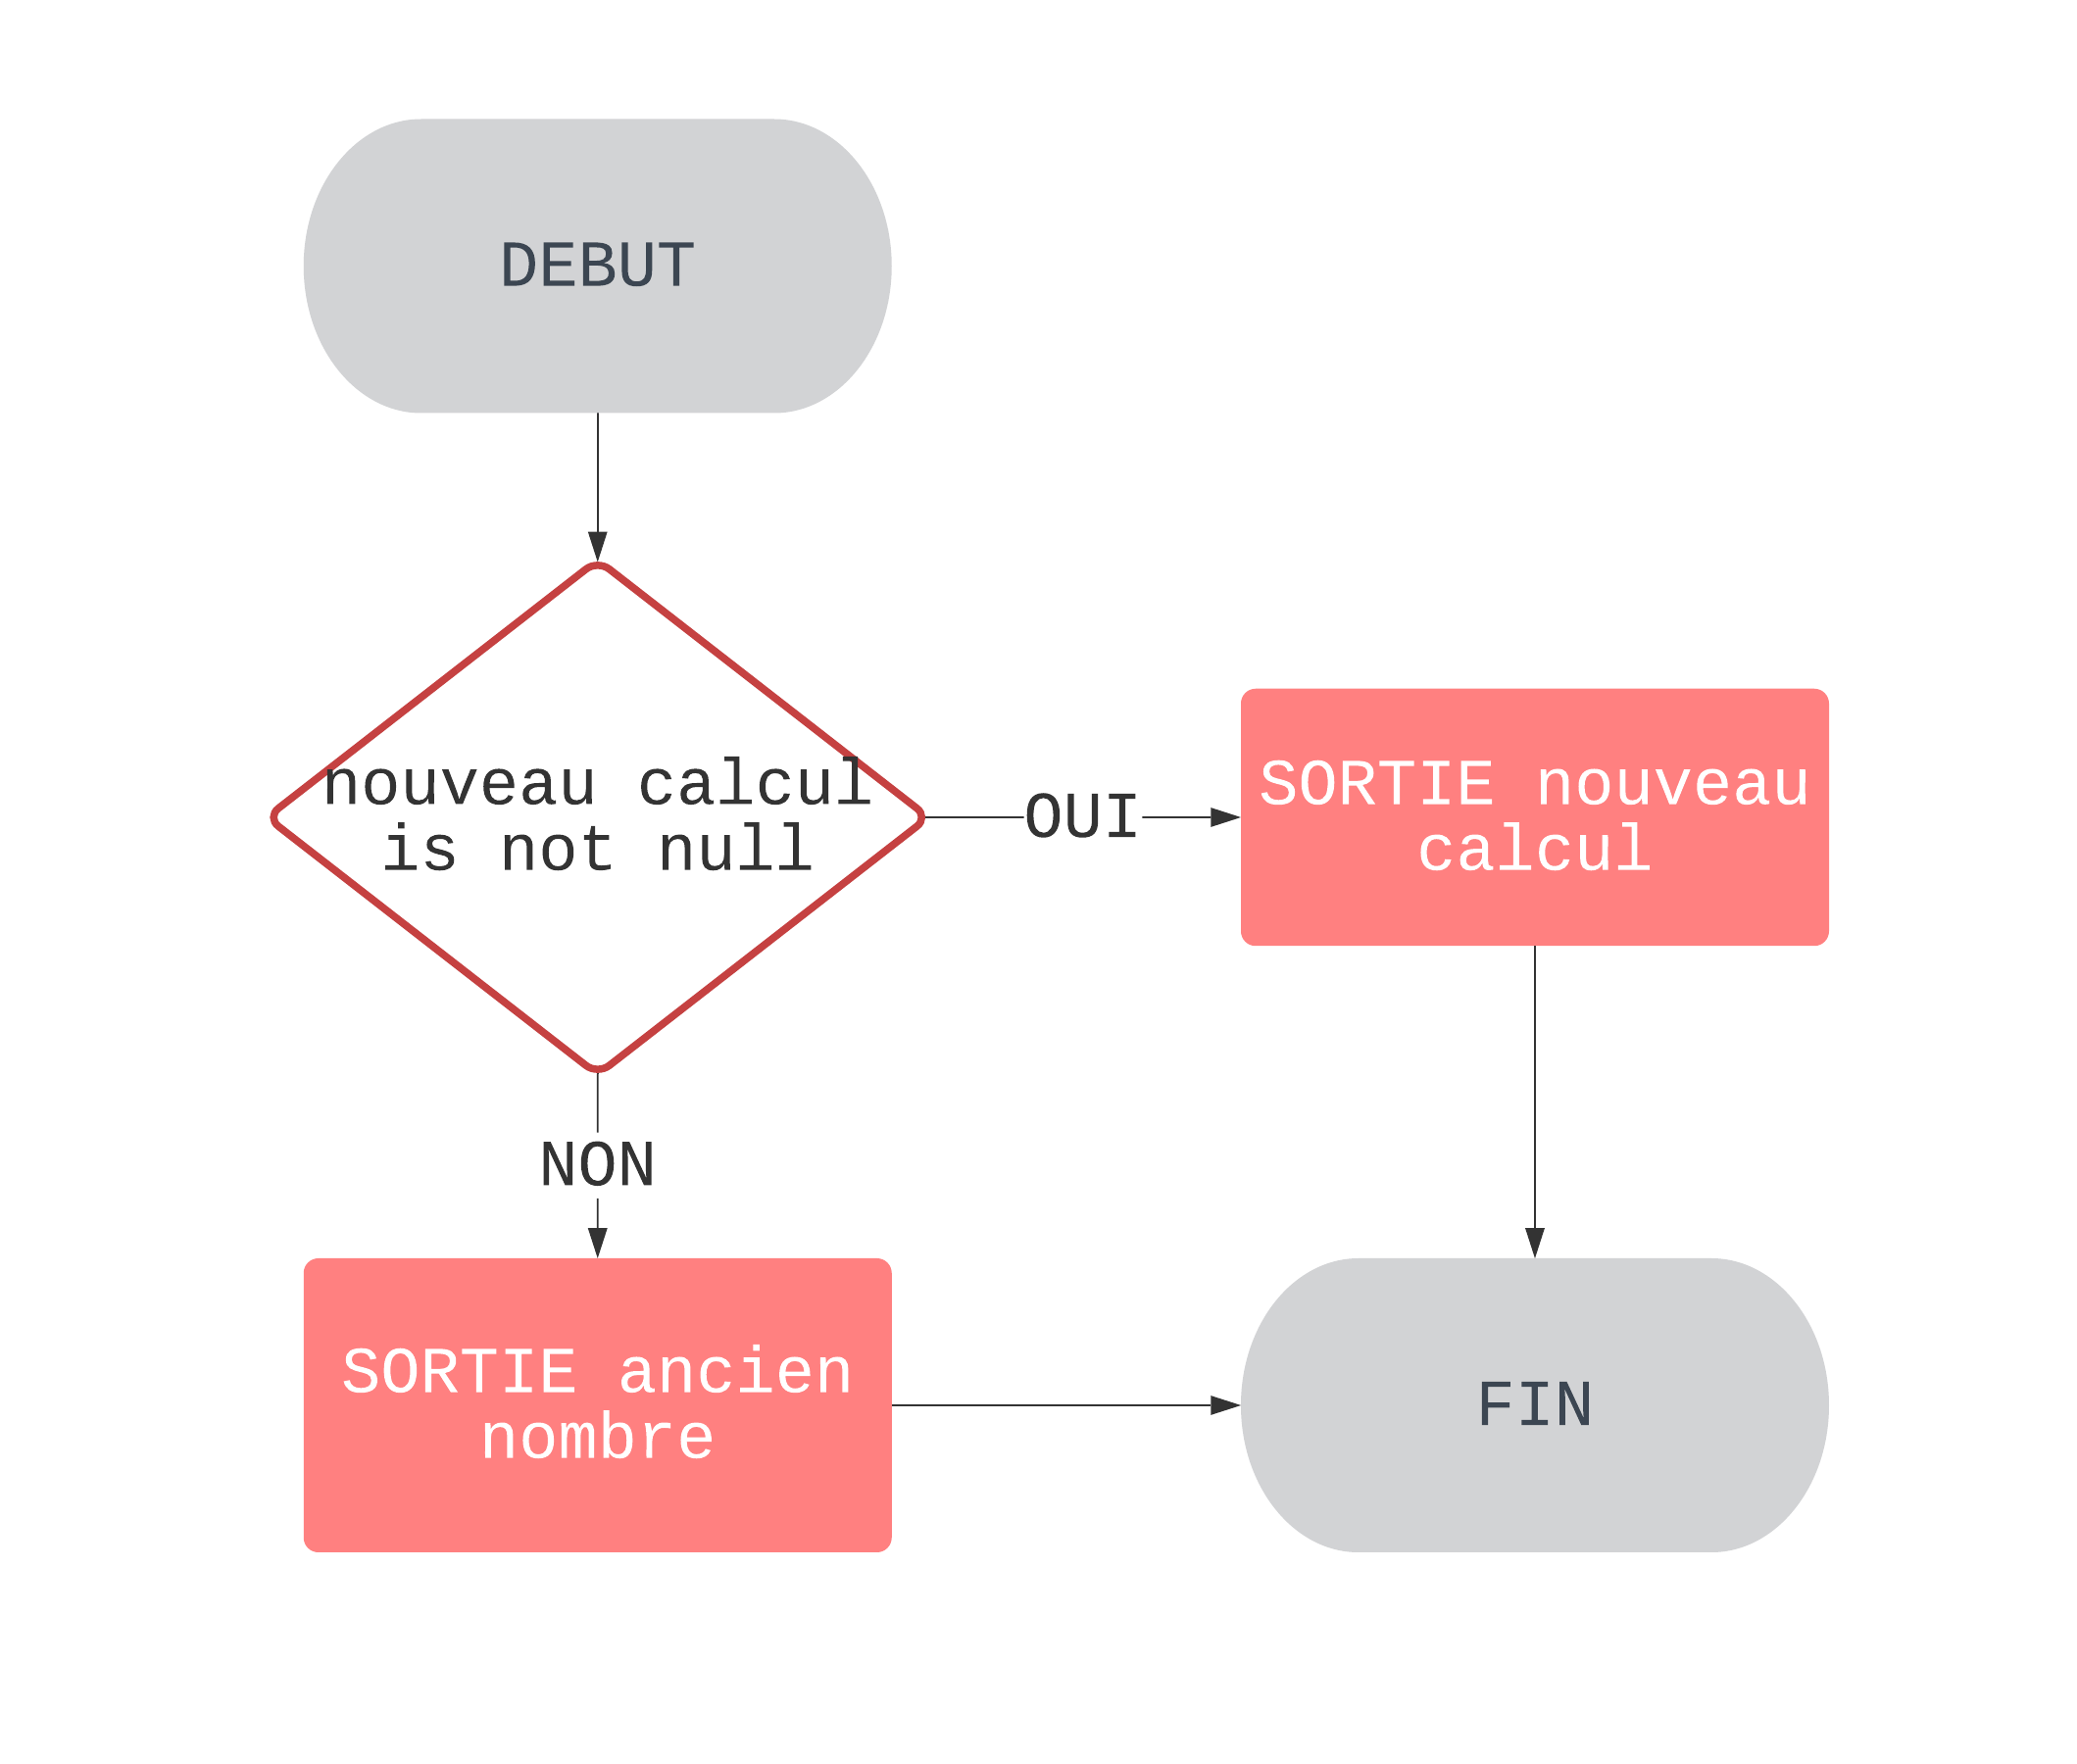
\includegraphics[scale=0.12]{Static/Algo_nombre_victimes.png} 
      \end{center}
        \caption{Algorigramme de fiabilisation du nombre de victime}  \label{fig:xray}
\end{figure}

Avec ces nouvelles valeurs, nous avons proc\'ed\'e au redressement de la nature du sinistre. Si le nombre de bless\'es ou de morts est sup\'erieur \`a z\'ero (0) alors on a un sinistre de nature 'Corporel'. Sinon si la charge est inf\'erieure ou \'egale \`a 100 000 dirham marocain et que le sinistre \'etait pr\'ec\'edemment qualifi\'e de 'Corporel' on le re-affecte en 'Materiel'. En effet, il n'y a aucune raison de le considérer comme un sinistre de nature 'Corporel'. Par contre, si aucune des conditions pr\'ec\'edentes n'est respect\'ee et on a la charge qui est strictement sup\'erieure \`a 100 000 dirham marocain ou un sinistre de nature 'Materiel' alors on conserve la valeur de la variable initiale '\textit{Nature\_Sinistre}'. Cet algorithme de redressement conduit \`a la cr\'eation d'une nouvelle variable '\textit{Nature\_Sinistre\_New}'.
\begin{figure}[H]
    \begin{center}
      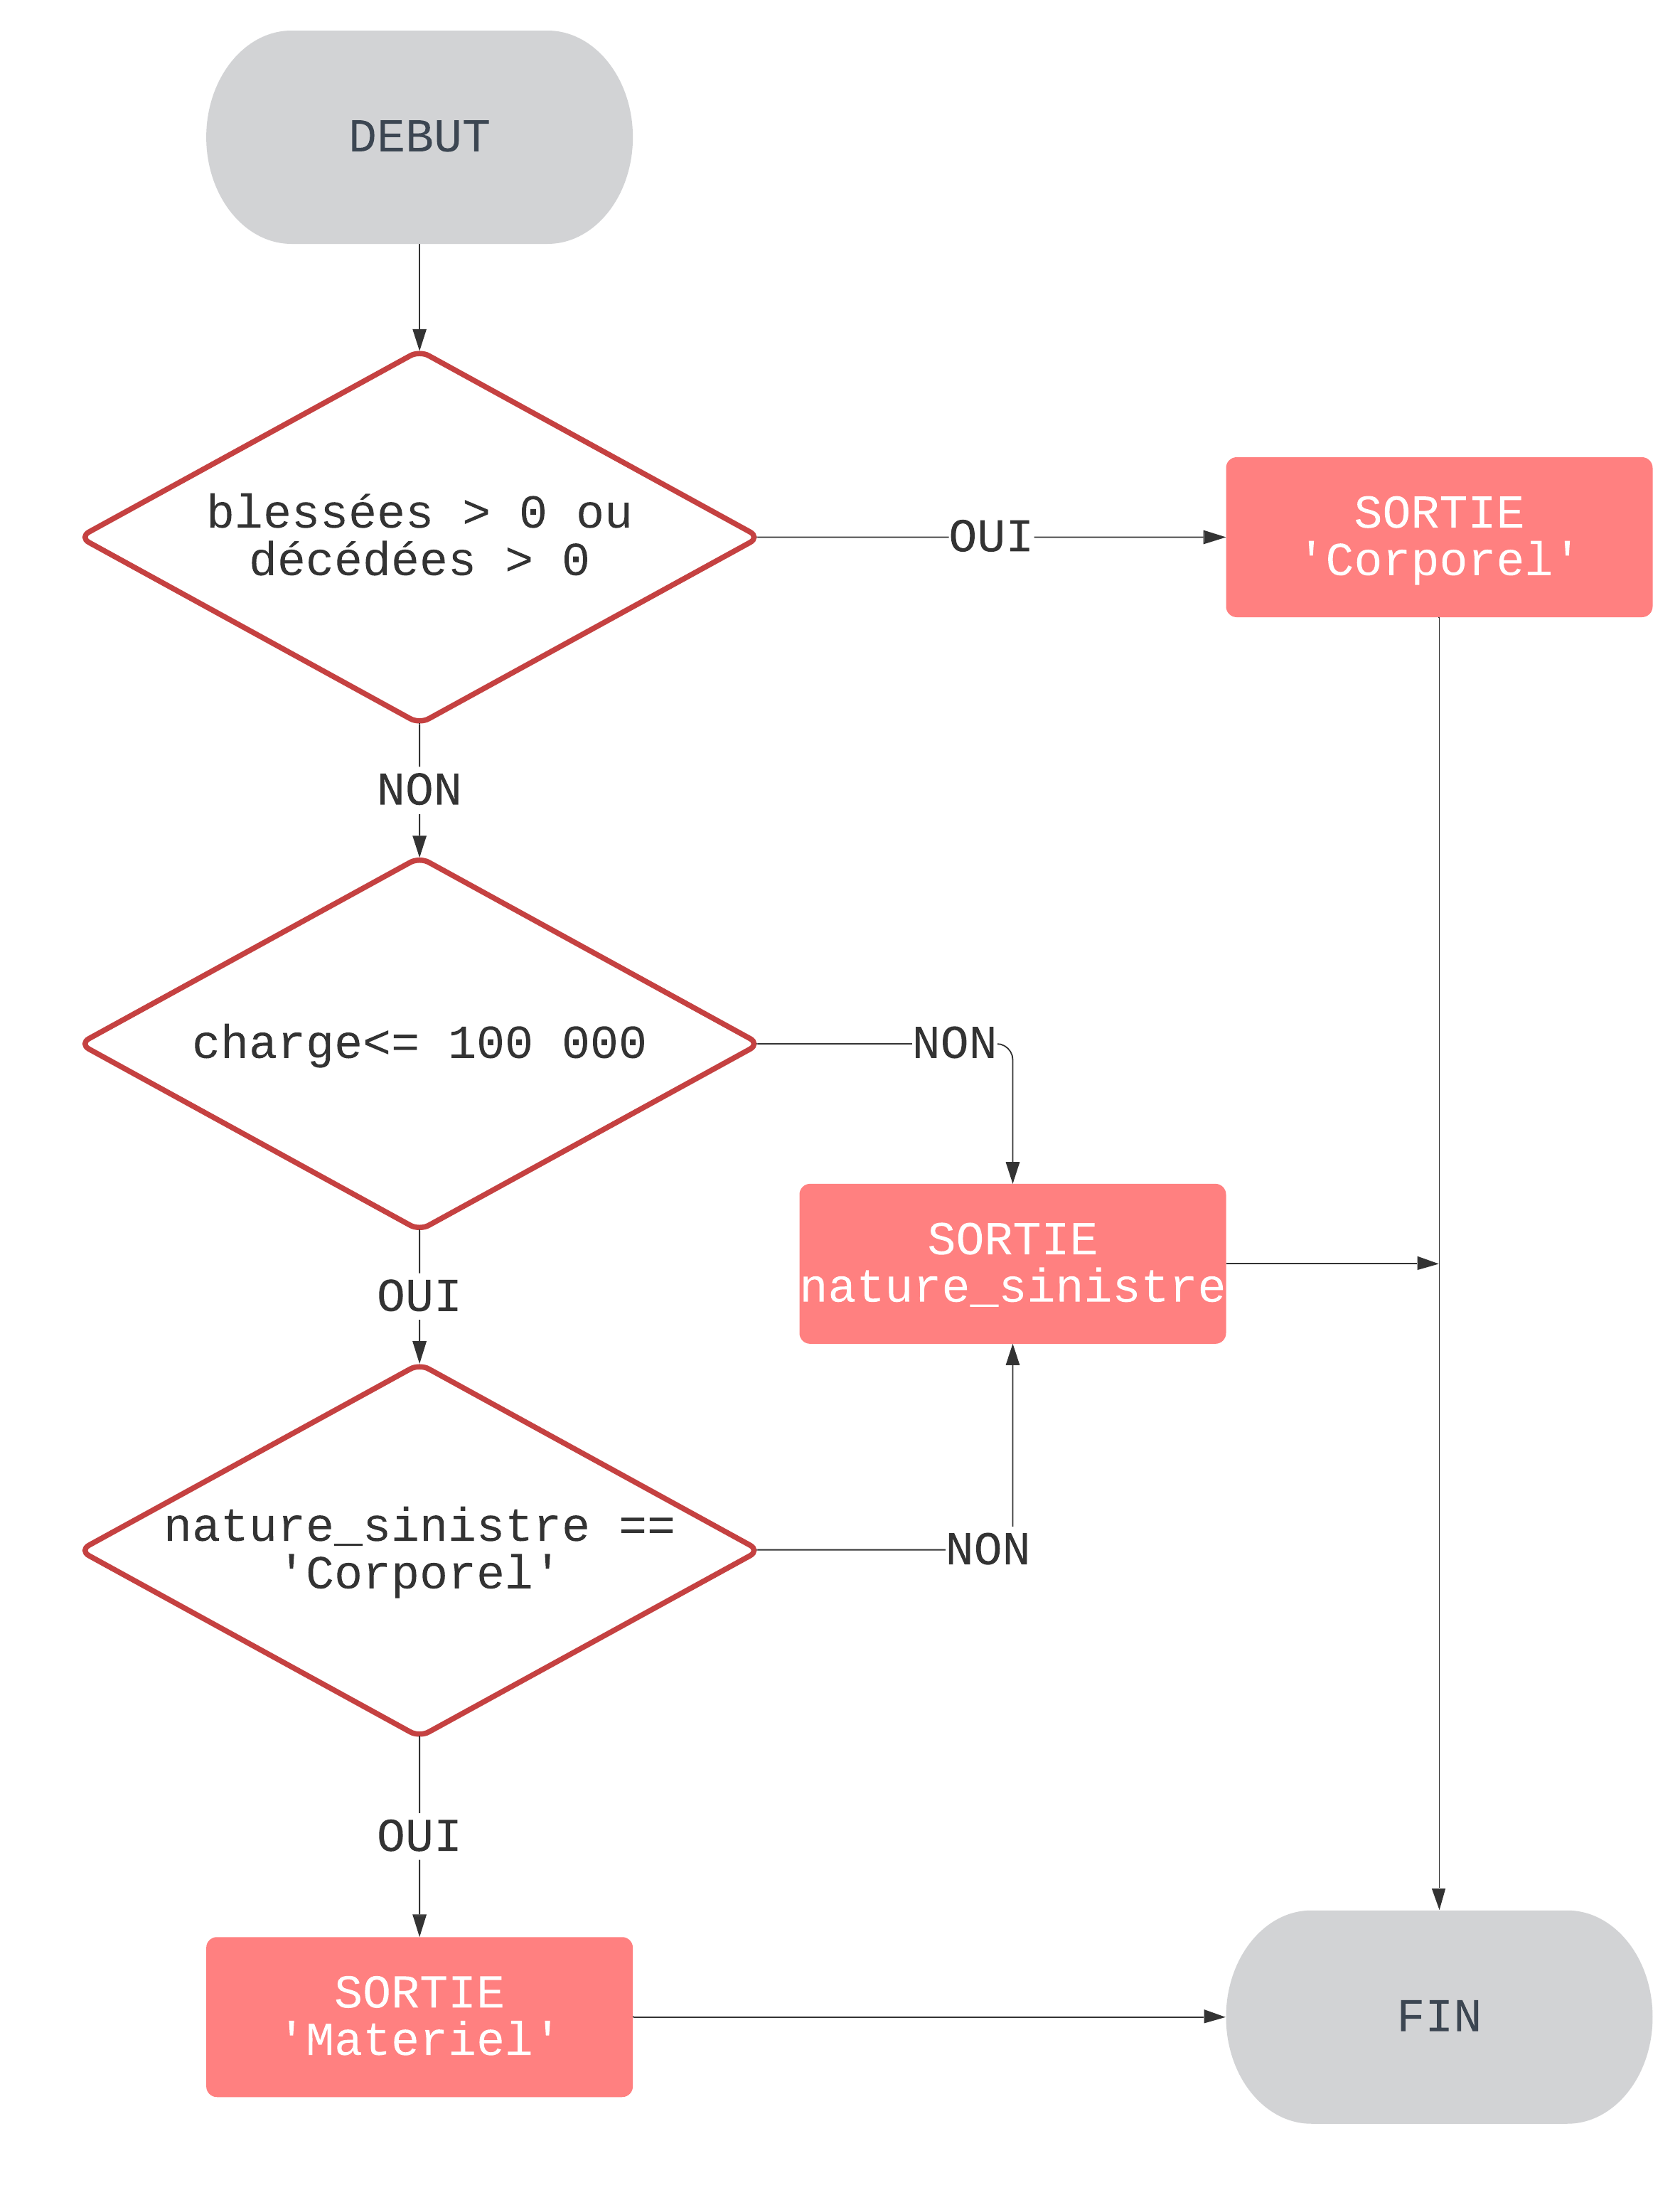
\includegraphics[scale=0.12]{Static/Algo_nature_sinistre.png} 
      \end{center}
        \caption{Algorigramme de fiabilisation de la nature du sinistre}  \label{fig:xray}
\end{figure}

\subsection{Algorithme de correction des probl\`emes d'encodages}
Les cibles de notre correction sont les mots du dictionnaire (pas les noms propres). L'algorithme utilis\'e se sert de la distance de Levenshtein pour identifier les corrections orthographiques les plus probables pour un mot : il s'agit des mots candidats. La distance de Levenshtein est une mesure de similarit\'e entre deux chaînes de caract\`eres. Elle est \'egale au nombre d'op\'erations \'el\'ementaires \`a r\'ealiser  pour transformer une chaîne M en une chaîne P. Il s'agit de :
\begin{itemize}[parsep=0cm,itemsep=0cm]
\item la substitution d'un caract\`ere;
\item l'insertion  ou l'ajout d'un caract\`ere;
\item la suppression ou l'effacement d'un caract\`ere.
\end{itemize}
Une fois la liste des mots candidats obtenue, l'algorithme compare ensuite tous les candidats à un dictionnaire de mots. La particularit\'e de ce dictionnaire est qu'il associe \`a chaque mot une fr\'equence d'apparition. La cl\'e est le mot et la valeur est la fr\'equence du mot. Le candidat ayant la plus forte fr\'equence d'apparition est plus susceptible d'être le résultat correct. En cas de co-occurrence un classement par ordre alphab\'etique est effectu\'e. Cet algorithme est impl\'ement\'e en Python par la biblioth\`eque SpellChecker. L'algorigramme mis en oeuvre pour corriger nos anomalies est le suivant : 
\begin{figure}[H]
    \begin{center}
      \includegraphics[scale=0.50]{Static/algo_spellchecker.png} 
      \end{center}
        \caption{Algorigramme de correction d'orthographe}  \label{fig:xray}
\end{figure}

\subsection{Fiabilisation des variables indicatrices}
Tout montant strictement sup\'erieur \`a z\'ero (0) doit \^etre mat\'erialis\'e par la modalit\'e 'Y' au niveau de la variable indicatrice. La correction de ces incoh\'erences est donc faite \`a l'aide de l'algorithme suivant: si le montant est sup\'erieur \`a  z\'ero (0), on affecte \`a une nouvelle variable indicatrice la valeur 'Y'. Dans le cas contraire, c'est la valeur 'N' qui est retournée afin de signifier qu'il n'y a pas de frais. La correction aboutit \`a la cr\'eation d'une nouvelle colonne afin de ne pas alt\'erer les donn\'ees existantes. L'algorithme mis en place \`a permis de corriger les incoh\'erences et d'imputer les valeurs manquantes des variables indicatrices.
%\newpage
\begin{figure}[H]
    \begin{center}
      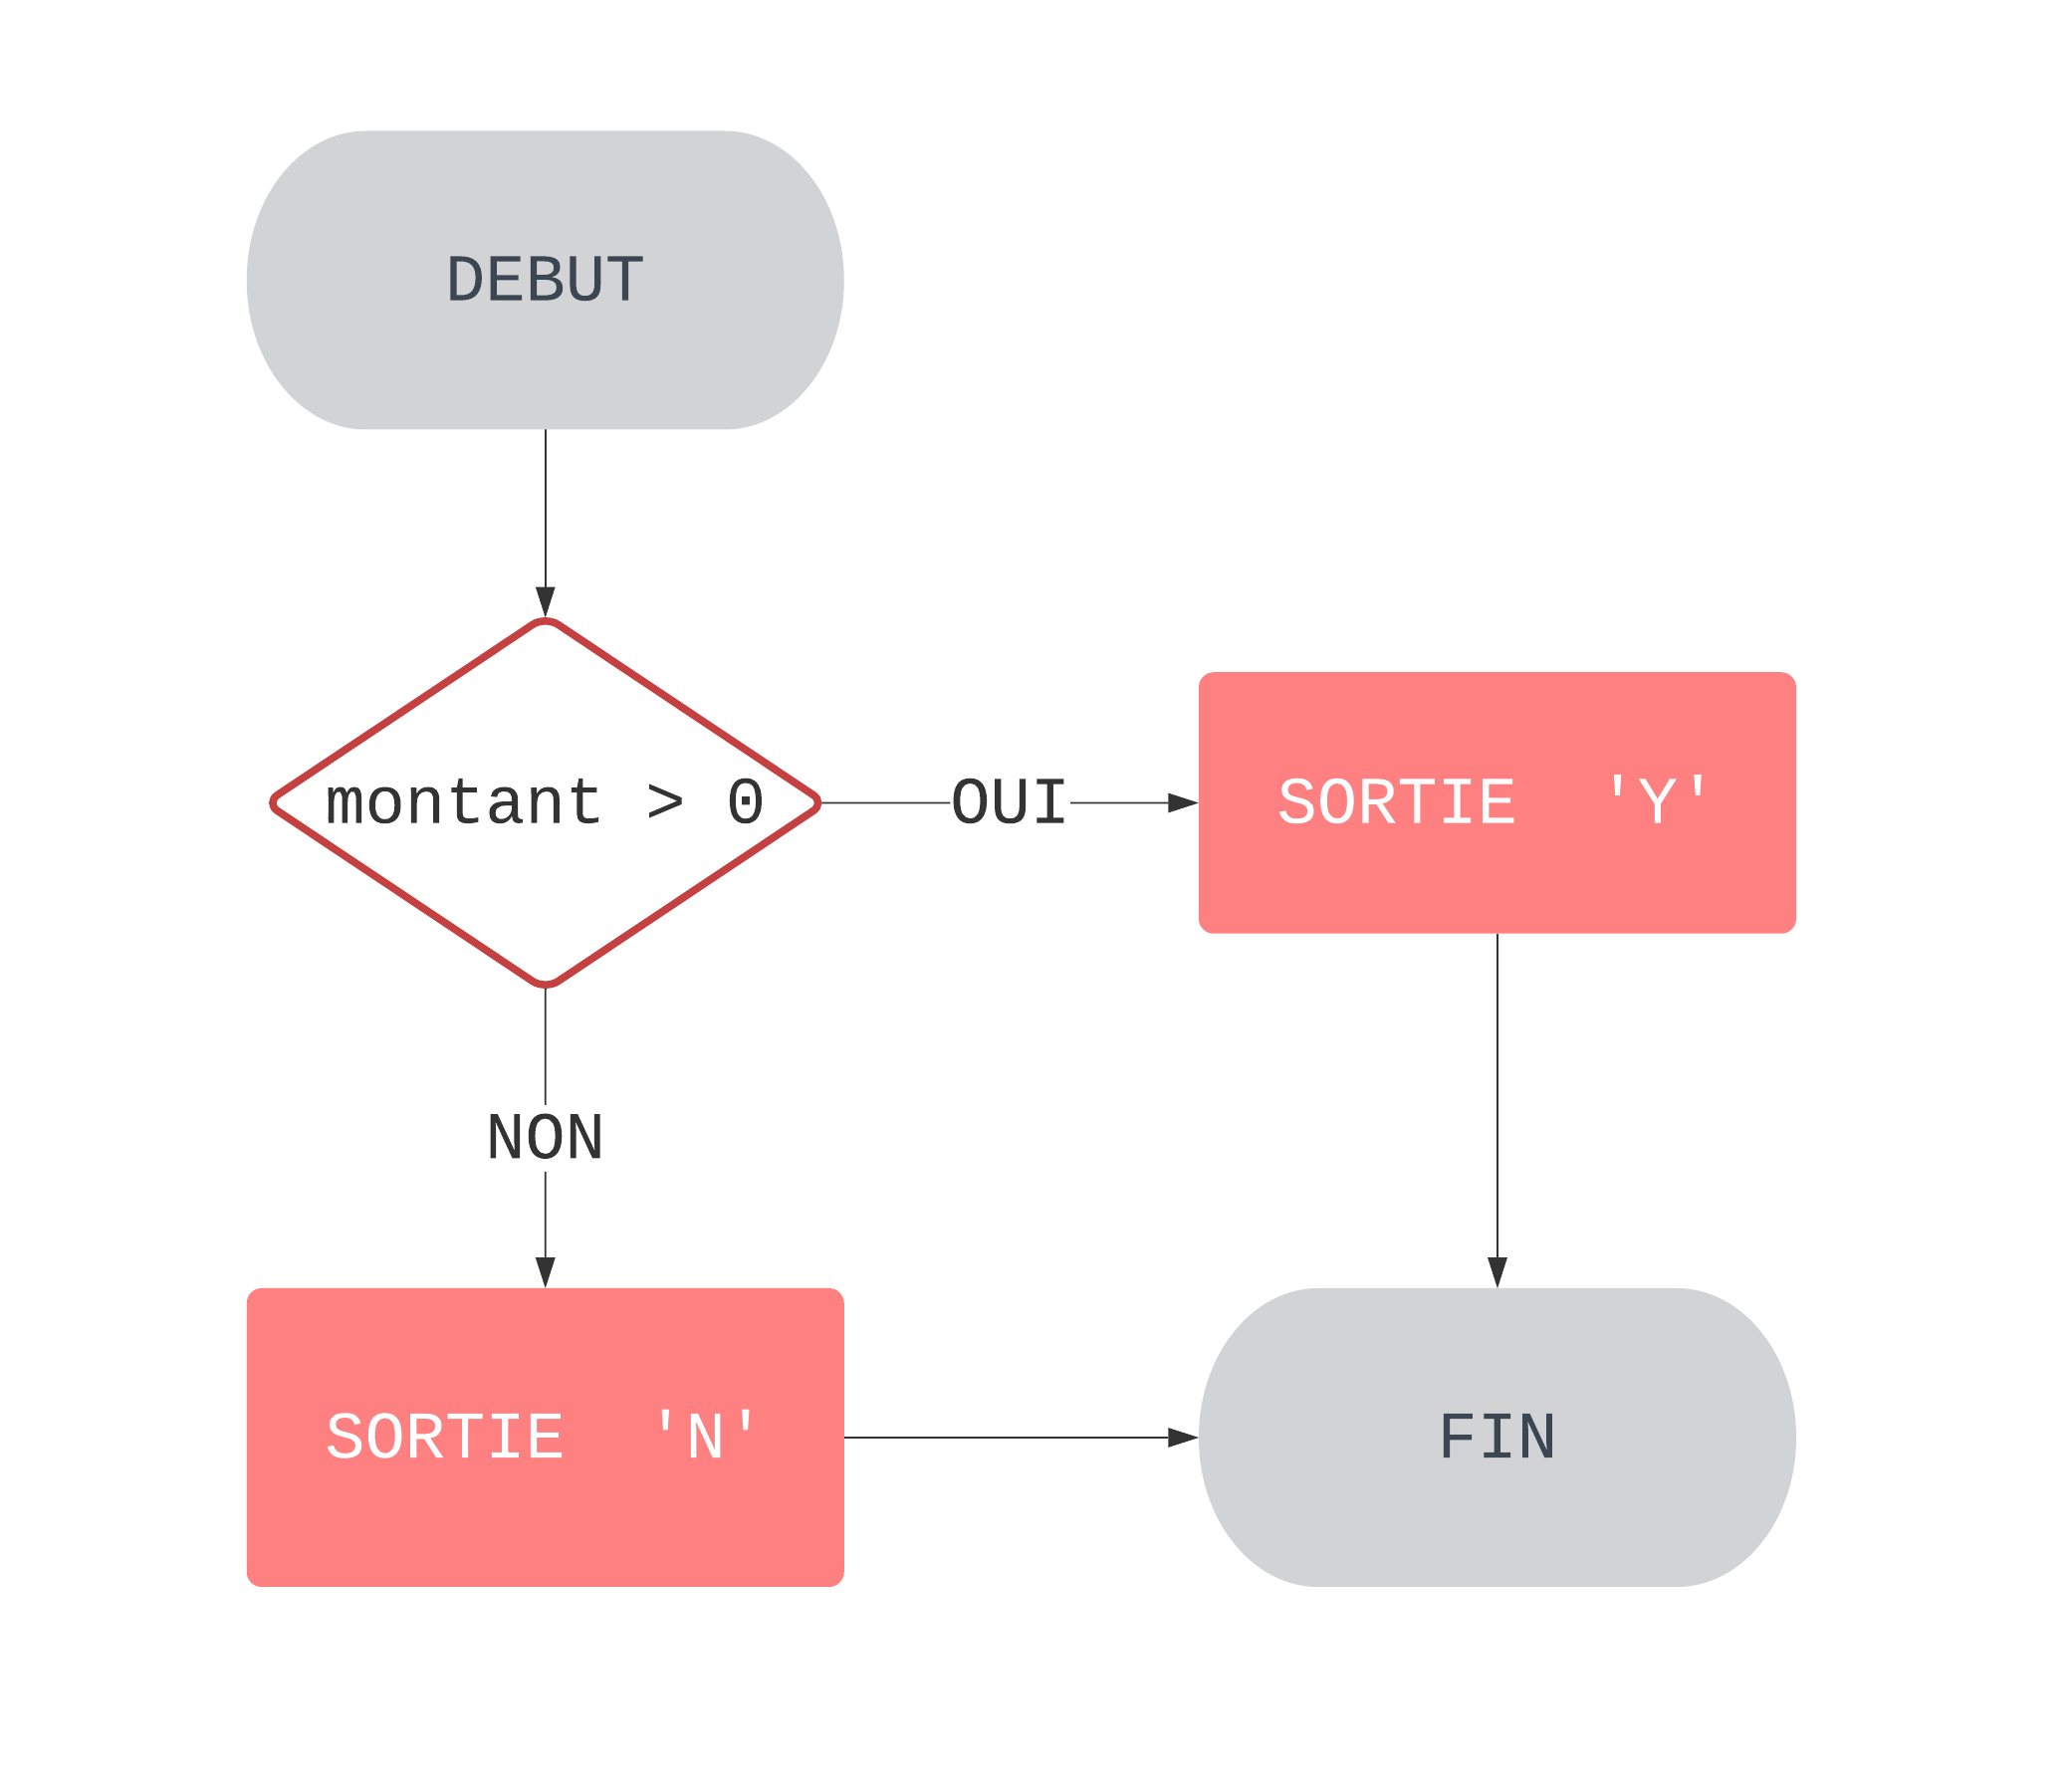
\includegraphics[scale=0.12]{Static/Algorithm_INDICATRICE.png} 
      \end{center}
        \caption{Algorigramme de r\'esolution des incoh\'erences variable indicatrice - montant}  \label{fig:xray}
\end{figure}
